%------------------------------------------------------------------------------
\section{Smoothed estimating equation estimator}\label{sec:see_method}
%------------------------------------------------------------------------------
The basic idea of smoothd estimating equation (SEE) estimator for the IVQR
model is to replace the indicator function in the moment condition with a smooth
function. To be precise, we replace the moment condition in Equation
(\ref{eq:moment2}) with
\begin{align}
\frac{1}{n}\sum_{i=1}^n \left[ \tau - \Is (Y_i  - \Db_i'\alphab - \Xb_i'\betab
\leq 0) \right] \Psib_i(\Xb, \Zb) = 0 \label{eq:moment_sgmm}
\end{align}
where $\Is()$ is defined as
\begin{align}
\Is(v) & =
\begin{cases}
  1 & \text{if $v \leq -1$} \\
  0 & \text{if $v \geq 1$}\\
  \frac{1-v}{2} &\text{if $-1 < v < 1$}
\end{cases}
\label{eq:Is}
\end{align}
Mathematically, $\Is() = \max\{0, \min\{1, \frac{1-v}{2}\}\}$.

Figure \ref{fig:sgmm} plot the $\Is(v/h)$ with different bandwidth $h$. We see
that smaller bandwidth approximate the indicator function better.

\begin{figure}[H]
\caption{Smoothed indicator function}
\label{fig:sgmm}
\centering
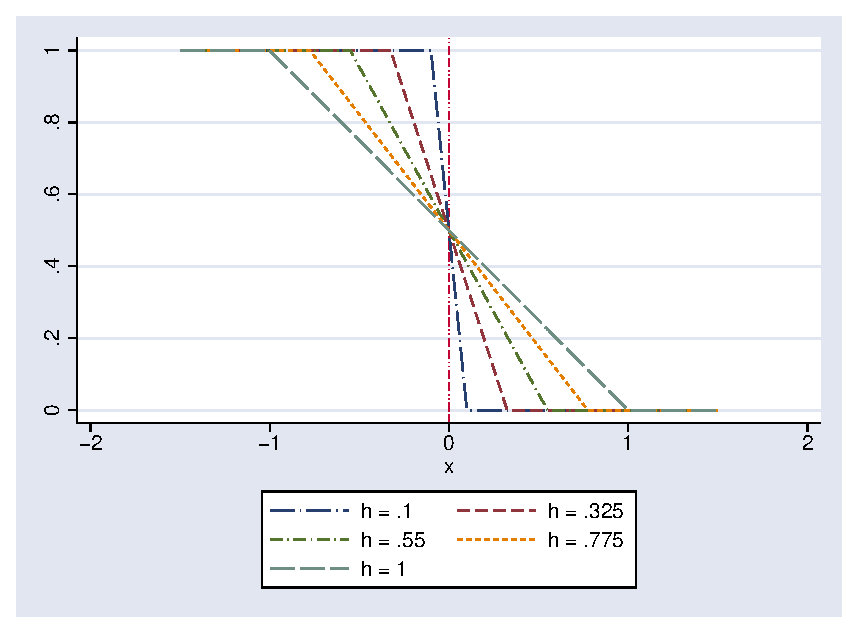
\includegraphics[scale=0.8]{eps/i_sgmm}
\end{figure}

Here are some remarks on the smoothed EE estimator.

\begin{itemize}
  \item In practice, $\Psib(\Xb, \Zb) = (\Xb', \Phib(\Xb, \Zb)')'$, and
    $\Phib(\Xb, \Zb)$ can be computed as the linear projection of $\Db$'s on the
    space spanned by $\Xb$ and $\Zb$. So, the over-identified model can 
    be transformed to a just-identified model. 

  \item Given a bandwidth $h$, the solution to Equation (\ref{eq:moment_sgmm})
    can be found via mata function {\ty solvenl()}. 

  \item The SEE estimator does not suffer from the curse of dimensionality as
    seen in the inverse quantile regression estimator.
\end{itemize}

%------------------------------------------------------------------------------
\subsection{Optimal bandwidth}
%------------------------------------------------------------------------------
The optimal bandwidth minimize the asymptotic MSE of the smoothed estimating
equations. For details, see Proposition 2 in \cite{Kaplan2017}.

The optimal bandwidth $\hsee$ is defined as
\begin{align}
  \hsee & = 
\left(
\frac{(r!)^2 \left[ 1- \int_{-1}^{1}G^2(u)du \right] f_U(0)}
{2r \left[\int_{-1}^1 G'(v)v^rdv \right]^2 
\left[f_U^{(r-1)}(0) \right]^2} \frac{p}{n}\right)^{\frac{1}{2r - 1}}
\end{align} 

where 
\begin{itemize}
  \item $G(u) = \Is(-u)$ 
  \item $r$ means $G(u)$ is a bounded $r$th order kernel such that $\int_{-1}^1
    v^k G'(v)dv = 0$ for $k = 1, 2, \ldots, r-1$ and $\int_{-1}^1 |v^r G'(v)dv|
    < \infty$. In the case of $\Is()$, $r = 2$.
  \item $p$ is the sum of the dimension of $\betab$ and $\alphab$.
  \item $U = Y - \Db'\alphab - \Xb'\betab$ and $f_U(0)$ is the PDF of
    $U$ at the point $0$.
  \item $f^{(1)}_U(0)$ is the derivatives of the PDF of $U$ evaluated at the
    point $0$.
\end{itemize}

Given the definition of $\Is()$ in Equation (\ref{eq:Is}), we can further
simplify the expression of $\hsee$. In particular,
\begin{align*}
1- \int_{-1}^{1}G^2(u)du 
&= 1 - \int_{-1}^1 \frac{(1 + v)^2}{4}dv = 1 - \frac{(1+v)^3}{12}|_{-1}^{1}
= \frac{1}{3} \\
\left[ \int_{-1}^1 G'(v)v^rdv  \right]^2
&=\left[ \int_{-1}^1 \frac{v^2}{2}dv \right]^2  
= \left[ \frac{v^3}{6}|_{-1}^1 \right]^2
= \left[ \frac{1}{6} - \frac{-1}{6} \right]^2 = \frac{1}{9}
\end{align*}
Plug in these two values into $\hsee$, we have
\begin{align}
  \hsee & = 
\left(
\frac{(2!)^2 \frac{1}{3}f_U(0)}
{2*2 \frac{1}{9} 
\left[f_U^{(2-1)}(0) \right]^2} \frac{p}{n}\right)^{\frac{1}{2*2 - 1}} \nonumber
\\
&= 
\left(
\frac{3f_U(0)}{\left[f_U^{'}(0) \right]^2} \frac{p}{n}\right)^{\frac{1}{3}} 
\nonumber \\
&= \left( \frac{3p}{n} \right)^{\frac{1}{3}} 
\left(\frac{f_U(0)}{\left[f'_U(0)\right]^2} \right)^{\frac{1}{3}}
\label{eq:bwopt}
\end{align}
Notice that the term $\left( \frac{3p}{n} \right)^{\frac{1}{3}}$ can be used as
an initial value of the bandwidth. We can nonparametrically or parametrically
estimate $f_U(0)$ and $f_U'(0)$. 

%------------------------------------------------------------------------------
\subsection{Nonparametrically estimated optimal bandwidth}
%------------------------------------------------------------------------------
The optimal bandwidth in Equation (\ref{eq:bwopt}) requires the evaluation of
$f_U(0)$ and $f_U'(0)$. Both terms can be estimated using a Kernel-based method.

For $f_U(0)$, given an initial estimate of residuals $\hat{u_i} = Y_i 
-\Db_i'\hat{\alphab}(\tau) -\Xb_i'\hat{\betab}(\tau)$, the kernel density
estimator is 
\begin{align}
  \frac{1}{ns}\sum_{i=1}^n K(\frac{-\hat{u}_i}{s})
\end{align}
where $s$ is the kernel bandwidth and $K()$ is the Gaussian Kernel.

Following the point-wise optimal bandwidth approach in \cite{DasGupta2008} and the
Gaussian reference approach in \cite{Silverman1998}, the optimal $s^*$ is

\begin{align}
  s^* = \left(\frac{1}{2n\sqrt{\pi}}\right)^{1/5}
  \sigma \left\{\phi(\Phi^{-1}(\tau))
  [\left( \Phi^{-1}(\tau) \right)^2 - 1 ]^2 \right\}^{-1/5}
\end{align}
where $\phi()$ is standard Normal density function and $\Phi()$ is standard
Normal CDF. $\sigma$ can be replaced by the sample deviation of the $\hat{u}$
or the standard normal interquartile range, whichever is smaller. 

For the density derivative $f'_U(0)$, the kernel estimator is 
\begin{align}
  \frac{1}{nb^2} \sum_{i=1}^n K'(-\hat{u}_i/b)
\end{align}
, where $K'()$ is the derivative of the Gaussian Kernel.

Following \cite{Wand1995}, the optimal bandwidth $b^*$ can be estimated as 
\begin{align}
b^* =  n^{-1/7}\sigma
\left(
\frac{3/(4\sqrt{\pi})}{
\phi(\Phi^{-1}(\tau)) 
\left[
\Phi^{-1}(\tau)
\right]^2
\left[3 - [\Phi^{-1}(\tau)]^2 \right]^2
}
\right)^{1/7}
\end{align}


%------------------------------------------------------------------------------
\subsection{Parametrically estimated optimal bandwidth}
%------------------------------------------------------------------------------
The optimial bandwidth in Equation (\ref{eq:bwopt}) can also be estimated
parametrically. Assuming the residuals $u$ follows a specific distribution,
the terms $f_U(0)$ and $f'_U(0)$ can be computed.

Suppose $u$ follows a Gaussian distribution, the optimal bandwidth can be
simplified as
\begin{align}
  \hsee =
  n^{-1/3}\sigma
  \left(
  	\frac{3 k_d}
	{
	  \{\Phi^{-1}(\tau)\}^2 \phi(\Phi^{-1}(\tau))
      }
      \right)^{1/3}
\end{align}


%------------------------------------------------------------------------------
\subsection{Detection of ``bad'' bandwidth}
%------------------------------------------------------------------------------
Given any bandwidth $h$, the SEE estimator may or may not converge. A ``bad''
bandwidth means that the SEE estimator does not converge or the SEE estimator
converges, but the point estimates are out of 95\% dual confidence interval. In
the first scenario, the non-convergence issue can be detected easily.  We can
employ the ``robust'' inference approach in \cite{Chernozhukov2008} in the
second scenario. For a detailed discussion, see Section \ref{sec:iqr_robust}.

In particular, we run an auxiliary quantile regression of $Y -
\Db'\hat{\alpha}_{SEE}$ on $\Xb$ and $\Phib(\Xb, \Zb)$, where
$\hat{\alpha}_{SEE}$ is SEE estimates for $\alphab$. Denote the $W_{h}$ as the
Wald statistic for the coefficient on $\Phib(\Xb, \Zb)$. If $W_h$ is greater
than the critical value $c_p$, the point estimates for the endogenous
coefficients are out of the $95\%$ confidence interval.



%------------------------------------------------------------------------------
\subsection{Variance-covariance estimation}
%------------------------------------------------------------------------------
The SEE estimator has the same (first-order) asymptotic distribution and
covariance structure as the inverse quantile regression estimator.  See the
second equation in Theorem 5 in \cite{DeCastro2019} for the derivation.  It
turns out that the SEE estimator in \cite{Kaplan2017} is a special case of the
\cite{DeCastro2019} when assuming the linear IVQR model.  The formulas for the
asymptotic variance estimator are the same as in Remarks \ref{iqr:dist} and
\ref{iqr:vce}. 

Bootstrap can also be used to compute the standard errors.
